\newif\ifglobal

%%%%%%%%%%%%%%%%%%%%%%%
%%% Compile to view %%%
%%%%%%%%%%%%%%%%%%%%%%%

%%%%%%%%%%%%%%%%%%%%%%%%%%%%%%%%%%%%%%%%%%%%%%%%%%%
%%% Readme:                                     %%%
%%% https://www.overleaf.com/read/bwdjvfjksvjy/ %%%
%%%%%%%%%%%%%%%%%%%%%%%%%%%%%%%%%%%%%%%%%%%%%%%%%%%

% >>> M?: marks a module setting number or important notice

% >>> M4: Set {./relative-path} to external files for this module <<<
\def \modulefiles {./17-INTMTRX}
% To add an external file, use:
% (Replace '---' with actual filename)
% '\input{\modulefiles/tables/---.tex}' for tables
% '\includegraphics{\modulefiles/figures/---}' for figures
% '\subfile{\modulefiles/---}' for register files


% >>> M1: This module is in global project? <<<
% 'YES' - uncomment; 'NO' - comment out
\globaltrue

\ifglobal
    \documentclass[main\_\_CN.tex]{subfiles}
   
\else
    % Font "FandolSong-Regular" used by ctex does not have GSUB table.
    % It causes warnings that do not affect compilation and can be ignored.
    \PassOptionsToPackage{quiet}{fontspec}

    \documentclass[openany, 10pt]{book}
   
    % >>> M2: In ./00-shared/preamble-trm-module, also find
    %         settings for visibility of todo notes, watermark <<< 
    \usepackage{preamble-trm-module}


    % Enable Chinese typesetting
    \usepackage{ctex}

    % >>> M3: Temporary labels in Chinese
    %         you can add your own labels there <<<
    \myexternaldocument{./00-shared/temp-labels-cn}

\fi %\ifglobal


\setcounter{secnumdepth}{4}


% >>> M5: If this module needs any updates in
% './00-shared/preamble-trm-module.sty'
% (include additional package, etc.), contact your module PM
% or create the file './00-shared/changelog.tex' make the
% necessary updates yourself and document them in this file <<<


\begin{document}


% Sets language into which pre-defined bits of text are translated
\selectlanguage{chinese}

% Do not delete this block
\ifglobal
% Add the following front matter if
% this module is outside of global project
\else
    \InputIfFileExists{readme}{}{}
    {\let\clearpage\relax \listoftodos}
    \tableofcontents
    %\listoftables
    %\listoffigures
\fi

%%%%%%%%%%%%%%%%%%%%%%%%%
%%% Chapter status: this is the latest document. Please update this document directly if there is any updates in future%%%
%%%%%%%%%%%%%%%%%%%%%%%%%



%%%%%%%%%%%%%%%%%%%%%%%%%
%%% TRM Module Begins %%%
%%%%%%%%%%%%%%%%%%%%%%%%%
\hypertarget{intmtrx}{}
\chapter{中断矩阵 (INTERRUPT)}
\label{mod:intmtrx}



\section{概述}

\chipname{} 中断矩阵将任一外部中断源单独映射到 ESP-RISC-V CPU 的任一外部中断上，以便在外设中断信号产生后，及时通知 CPU 进行处理。

\chipname{} 有 62 个外部中断源，但 CPU 只支持 31 个中断。因此，将这些外部中断源映射至 CPU 中断必须使用中断矩阵。

\begin{tiplisting}
本章节只涉及将外部中断源映射到 CPU 中断，关于中断配置、中断向量表、中断服务程序推荐处理机制请参考章节 \ref{mod:riscvcpu} \textit{\nameref{mod:riscvcpu}}。
\end{tiplisting}

\section{特性}

\begin{itemize}
    \item 接收 62 个外部中断源作为输入
    \item 生成 31 个 CPU 的外部中断作为输出
    \item 支持查询外部中断源当前的中断状态
    \item 支持配置 CPU 的中断优先级、中断类型、中断阈值以及中断使能
\end{itemize}

中断矩阵的结构如图 \ref{fig:interrupt-matrix-structure} 所示。

\begin{figure}[H]
    \centering
    {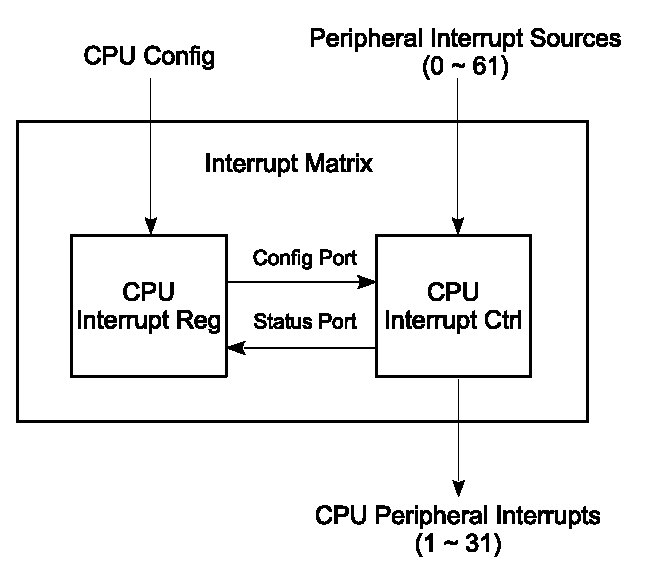
\includegraphics[width=0.5\textwidth]{17-INTMTRX/figures/17-INTMTRX-struct_20210705.eps}}
    \caption{中断矩阵结构图}
    \label{fig:interrupt-matrix-structure}
\end{figure}


\section{功能描述}

\subsection{外部中断源}

\chipname{} 共有 62 个外部中断源。表 \ref{tab:peripheral-interrupt-config-status-source} 列出了所有外部中断源，以及对应的中断配置寄存器与中断状态寄存器。

\begin{itemize}
    \item ``No."：表示外部中断源序号，范围：0 \verb+~+ 61
    \item ``章节"：详细描述外部中断源的章节
    \item ``中断源"：外部中断源名称
    \item ``配置寄存器"：用于将外部中断源分配至 CPU 外部中断
    \item ``状态寄存器"：用于读取中断源的中断状态
    \begin{itemize}
        \item ``状态寄存器 - 位"：表示在状态寄存器中的比特位置，用于记录相应中断源的状态 
        \item ``状态寄存器 - 名称"：表示状态寄存器的名称
    \end{itemize}
\end{itemize}



\clearpage
\begin{landscape}

\begin{footnotesize}
\begin{longtable}[c]{|*{6}{l|C{4cm}|C{3.5cm}|C{9.4cm}|p{0.3cm}|C{5.3cm}|}}
    \caption{CPU 外部中断配置寄存器、外部中断状态寄存器、外部中断源}
    \label{tab:peripheral-interrupt-config-status-source}\\
    
    \hline
     \rowcolor{gray!25}
    & & & & \multicolumn{2}{c|}{\textbf{状态寄存器}} \\
    \cline{5-6}
    \rowcolor{gray!25}
    \multirow{-2}*{\textbf{No.}} & \multirow{-2}*{\textbf{章节}} & \multirow{-2}*{\textbf{中断源}} & \multirow{-2}*{\textbf{配置寄存器}} & \textbf{位} & \textbf{名称} \\
    \hline
    \endfirsthead
    
    \hline
    \rowcolor{gray!25}
    & & & & \multicolumn{2}{c|}{\textbf{状态寄存器}} \\
    \cline{5-6}
    \rowcolor{gray!25}
    \multirow{-2}*{\textbf{No.}} & \multirow{-2}*{\textbf{章节}} & \multirow{-2}*{\textbf{中断源}} & \multirow{-2}*{\textbf{配置寄存器}} & \textbf{位} & \textbf{名称} \\
    \hline
    \endhead
    \endfoot
    

0 & 保留 & 保留 & 保留 & 0 & \multirow{32}*{\makecell{\hyperref[regdesc:INTERRUPTCORE0INTRSTATUS0REG]{INTERRUPT\_CORE0\_INTR\_STATUS\_0\_REG}}}                        	\\
    \cline{1-5}                                           
    1 & 保留 & 保留 & 保留 & 1 & \\
    \cline{1-5}                                           
    2 & 保留 & 保留 & 保留 & 2 & \\
    \cline{1-5}  
    3 &  保留 & 保留 & 保留 & 3 &                          	\\
    \cline{1-5}
    4 & 保留 & 保留 & 保留 & 4 &                          	\\
    \cline{1-5}
    5 & 保留 & 保留 & 保留 & 5 &                          	\\
    \cline{1-5}
    6 & 保留 & 保留  & 保留 & 6 &                          	\\
    \cline{1-5}
    7 & 保留 & 保留 & 保留 & 7 &                          	\\
    \cline{1-5}
    8 & 保留 & 保留 & 保留 & 8 &                          	\\
    \cline{1-5}
    9 & 保留 & 保留 & 保留 & 9 &                          	\\
    \cline{1-5}
    10 &  保留 & 保留 & 保留 & 10 &                          	\\
    \cline{1-5}
    11 &  保留 & 保留 & 保留 & 11 & \\
    
    \cline{1-5}
     12 &  保留 & 保留 & 保留 & 12 & \\
    
    \cline{1-5}
    
     13 &  保留 & 保留 & 保留 & 13 & \\
    \cline{1-5}
    
      14 &  保留 & 保留 & 保留 & 14 & \\
    \cline{1-5}
    
    15 & \textit{\nameref{mod:uart}} & UHCI0\_INTR & \hyperref[regdesc:INTERRUPTCORE0UHCI0INTRMAPREG]{INTERRUPT\_CORE0\_UHCI0\_INTR\_MAP\_REG} & 15 &                          	\\
    \cline{1-5}
    16 & \textit{\nameref{mod:iomuxgpio}} & GPIO\_PROCPU\_INTR & \hyperref[regdesc:INTERRUPTCORE0GPIOINTERRUPTPROMAPREG]{INTERRUPT\_CORE0\_GPIO\_INTERRUPT\_PRO\_MAP\_REG} & 16 &                          	\\
    \cline{1-5}
    17 & 保留 & 保留 & 保留 & 17 &                          	\\
    \cline{1-5}
    18 & 保留 & 保留 & 保留 & 18 &                          	\\
    \cline{1-5}
    19 & \textit{\nameref{mod:spi}} & GPSPI2\_INTR\_2 & \hyperref[regdesc:INTERRUPTCORE0SPIINTR2MAPREG]{INTERRUPT\_CORE0\_SPI\_INTR\_2\_MAP\_REG} & 19 &                          	\\
    \cline{1-5}
    20 & \textit{\nameref{mod:i2s}} & I2S\_INTR & \hyperref[regdesc:INTERRUPTCORE0I2S1INTMAPREG]{INTERRUPT\_CORE0\_I2S\_INT\_MAP\_REG} & 20 &                          	\\
    \cline{1-5}
    21 & \textit{\nameref{mod:uart}} & UART\_INTR & \hyperref[regdesc:INTERRUPTCORE0UARTINTRMAPREG]{INTERRUPT\_CORE0\_UART\_INTR\_MAP\_REG} & 21 &                          	\\
    \cline{1-5}
    22 & \textit{\nameref{mod:uart}} & UART1\_INTR & \hyperref[regdesc:INTERRUPTCORE0UART1INTRMAPREG]{INTERRUPT\_CORE0\_UART1\_INTR\_MAP\_REG} & 22 &                          	\\
    \cline{1-5}
    
    
    
    23  & \textit{\nameref{mod:ledpwm}} & LEDC\_INTR  & \hyperref[regdesc:INTERRUPTCORE0LEDCINTMAPREG]{INTERRUPT\_CORE0\_LEDC\_INT\_MAP\_REG} & 23 &                          	\\
    \cline{1-5}
    24  & \textit{\nameref{mod:efuse}} & EFUSE\_INTR  & \hyperref[regdesc:INTERRUPTCORE0EFUSEINTMAPREG]{INTERRUPT\_CORE0\_EFUSE\_INT\_MAP\_REG} & 24 &                          	\\
    \cline{1-5}
    25  & \textit{\nameref{mod:twai}} & TWAI\_INTR & \hyperref[regdesc:INTERRUPTCORE0TWAIINTMAPREG]{INTERRUPT\_CORE0\_TWAI\_INT\_MAP\_REG} & 25 &                          	\\
    \cline{1-5}
    26  & \textit{\nameref{mod:usbserialjtag}} & USB\_SERIAL\_JTAG\_INTR  & \hyperref[regdesc:INTERRUPTCORE0USBINTRMAPREG]{INTERRUPT\_CORE0\_USB\_INTR\_MAP\_REG}  & 26 &                          	\\
    \cline{1-5}
    
    27 & \textit{\nameref{mod:lowpowm}} & RTC\_CNTL\_INTR &\hyperref[regdesc:INTERRUPTCORE0RTCCOREINTRMAPREG]{INTERRUPT\_CORE0\_RTC\_CORE\_INTR\_MAP\_REG} & 27 & \\
    \cline{1-5}
 
    28  & \textit{\nameref{mod:rmt}} &  RMT\_INTR & \hyperref[regdesc:INTERRUPTCORE0RMTINTRMAPREG]{INTERRUPT\_CORE0\_RMT\_INTR\_MAP\_REG} & 28  &                          	\\
    \cline{1-5}
    \cline{1-5}
    29  & \textit{\nameref{mod:i2c}} & I2C\_EXT0\_INTR  & \hyperref[regdesc:INTERRUPTCORE0I2CEXT0INTRMAPREG]{INTERRUPT\_CORE0\_I2C\_EXT0\_INTR\_MAP\_REG}  & 29  &                          	\\
    \cline{1-5}
    30 & 保留 & 保留 & 保留 & 30 & \\
    \cline{1-5}
     31 & 保留 & 保留 & 保留 & 31 & \\
    \hline
    
    32 & \textit{\nameref{mod:timg}} & TG\_T0\_INTR & \hyperref[regdesc:INTERRUPTCORE0TGT0INTMAPREG]{INTERRUPT\_CORE0\_TG\_T0\_INT\_MAP\_REG} & 0 &  \multirow{30}*{\makecell{\hyperref[regdesc:INTERRUPTCORE0INTRSTATUS1REG]{INTERRUPT\_CORE0\_INTR\_STATUS\_1\_REG}}}                    	
    \\\cline{1-5}
    33  & \textit{\nameref{mod:timg}} & TG\_WDT\_INTR & \hyperref[regdesc:INTERRUPTCORE0TGWDTINTMAPREG]{INTERRUPT\_CORE0\_TG\_WDT\_INT\_MAP\_REG}  &1  &                          	\\
    \cline{1-5}
    34  & \textit{\nameref{mod:timg}} & TG1\_T0\_INTR & \hyperref[regdesc:INTERRUPTCORE0TG1T0INTMAPREG]{INTERRUPT\_CORE0\_TG1\_T0\_INT\_MAP\_REG}  &2  &                          	\\
    \cline{1-5}
    35  & \textit{\nameref{mod:timg}} & TG1\_WDT\_INTR & \hyperref[regdesc:INTERRUPTCORE0TG1WDTINTMAPREG]{INTERRUPT\_CORE0\_TG1\_WDT\_INT\_MAP\_REG}  &3  &                          	\\
    \cline{1-5}
     36 & 保留 & 保留 & 保留 & 36 & \\
    \cline{1-5}
    37 & \textit{\nameref{mod:systimer}}  & SYSTIMER\_TARGET0\_INTR & \hyperref[regdesc:INTERRUPTCORE0SYSTIMERTARGET0INTMAPREG]{INTERRUPT\_CORE0\_SYSTIMER\_TARGET0\_INT\_MAP\_REG}  &5  &                          	\\
    \cline{1-5}
    38 & \textit{\nameref{mod:systimer}} & SYSTIMER\_TARGET1\_INTR &\hyperref[regdesc:INTERRUPTCORE0SYSTIMERTARGET1INTMAPREG]{INTERRUPT\_CORE0\_SYSTIMER\_TARGET1\_INT\_MAP\_REG}  & 6 &                            	\\
    \cline{1-5}
    39  & \textit{\nameref{mod:systimer}} & SYSTIMER\_TARGET2\_INTR &\hyperref[regdesc:INTERRUPTCORE0SYSTIMERTARGET2INTMAPREG]{INTERRUPT\_CORE0\_SYSTIMER\_TARGET2\_INT\_MAP\_REG}  &7  &                          	\\
    \cline{1-5}
    40  & 保留 & 保留 & 保留  &8  &                          	\\
    \cline{1-5}
    
    41 & 保留 & 保留 & 保留 & 9 &       	\\
    \cline{1-5}
    
    
    42 & 保留 & 保留 & 保留 & 10 & \\
    
    \cline{1-5}
    
    43 & \textit{\nameref{mod:sensor}} & vDIGTAL\_ADC\_INTR & \hyperref[regdesc:INTERRUPTCORE0APBADCINTMAPREG]{INTERRUPT\_CORE0\_APB\_ADC\_INT\_MAP\_REG}  & 11  &                          	\\
    \cline{1-5}
    44 & \textit{\nameref{mod:dma}} & GDMA\_CH0\_INTR  & \hyperref[regdesc:INTERRUPTCORE0DMACH0INTMAPREG]{INTERRUPT\_CORE0\_DMA\_CH0\_INT\_MAP\_REG}  &12  &                          	\\
    \cline{1-5}
    45 & \textit{\nameref{mod:dma}} & GDMA\_CH1\_INTR  & \hyperref[regdesc:INTERRUPTCORE0DMACH1INTMAPREG]{INTERRUPT\_CORE0\_DMA\_CH1\_INT\_MAP\_REG}  &13  &                          	\\
    \cline{1-5}
    46 & \textit{\nameref{mod:dma}} & GDMA\_CH2\_INTR  & \hyperref[regdesc:INTERRUPTCORE0DMACH2INTMAPREG]{INTERRUPT\_CORE0\_DMA\_CH2\_INT\_MAP\_REG}  &14  &                          	\\
    \cline{1-5}
    47 & \textit{\nameref{mod:rsa}} & RSA\_INTR  & \hyperref[regdesc:INTERRUPTCORE0RSAINTMAPREG]{INTERRUPT\_CORE0\_RSA\_INTR\_MAP\_REG}  &15  &                          	\\
    \cline{1-5}
    
    48 & \textit{\nameref{mod:aes}} & AES\_INTR  & \hyperref[regdesc:INTERRUPTCORE0AESINTMAPREG]{INTERRUPT\_CORE0\_AES\_INTR\_MAP\_REG}  &16  &                          	\\
    \cline{1-5}
    49 & \textit{\nameref{mod:sha}} & SHA\_INTR  & \hyperref[regdesc:INTERRUPTCORE0SHAINTMAPREG]{INTERRUPT\_CORE0\_SHA\_INTR\_MAP\_REG}  &17  &                          	\\
    \cline{1-5}
    50 & \textit{\nameref{mod:sysreg}} & SW\_INTR\_0  & \hyperref[regdesc:INTERRUPTCORE0CPUINTRFROMCPU0MAPREG]{INTERRUPT\_CORE0\_CPU\_INTR\_FROM\_CPU\_0\_MAP\_REG}  &18  &                          	\\
    \cline{1-5}
    51 & \textit{\nameref{mod:sysreg}} & SW\_INTR\_1  &\hyperref[regdesc:INTERRUPTCORE0CPUINTRFROMCPU1MAPREG]{INTERRUPT\_CORE0\_CPU\_INTR\_FROM\_CPU\_1\_MAP\_REG}  &19  &                          	\\
    \cline{1-5}
    52 & \textit{\nameref{mod:sysreg}} & SW\_INTR\_2 &\hyperref[regdesc:INTERRUPTCORE0CPUINTRFROMCPU2MAPREG]{INTERRUPT\_CORE0\_CPU\_INTR\_FROM\_CPU\_2\_MAP\_REG}  &20  &                          	\\
    \cline{1-5}
    53 & \textit{\nameref{mod:sysreg}} & SW\_INTR\_3 &\hyperref[regdesc:INTERRUPTCORE0CPUINTRFROMCPU3MAPREG]{INTERRUPT\_CORE0\_CPU\_INTR\_FROM\_CPU\_3\_MAP\_REG}  &21  &                          	\\
    \cline{1-5}
    54 & \textit{\nameref{mod:dbgassist}} & ASSIST\_DEBUG\_INTR  &\hyperref[regdesc:INTERRUPTCORE0ASSISTDEBUGINTRMAPREG]{INTERRUPT\_CORE0\_ASSIST\_DEBUG\_INTR\_MAP\_REG}  &22  &                          	\\
    \cline{1-5}
    55 & \textit{\nameref{mod:permctrl}} & PMS\_DMA\_VIO\_INTR  & \hyperref[regdesc:INTERRUPTCORE0DMAAPBPERIPMSMONITORVIOLATEINTRMAPREG]{INTERRUPT\_CORE0\_DMA\_APBPERI\_PMS\_MONITOR\_VIOLATE\_INTR\_MAP\_REG}  &23  &                          	\\
    \cline{1-5} 

    56 & \textit{\nameref{mod:permctrl}} & PMS\_IBUS\_VIO\_INTR  & \hyperref[regdesc:INTERRUPTCORE0CORE0IRAM0PMSMONITORVIOLATEINTRMAPREG]{INTERRUPT\_CORE0\_CORE\_0\_IRAM0\_PMS\_MONITOR\_VIOLATE\_INTR\_MAP\_REG}  &24  &                          	\\
    \cline{1-5}    
    
    57 & \textit{\nameref{mod:permctrl}} & PMS\_DBUS\_VIO\_INTR  & \hyperref[regdesc:INTERRUPTCORE0CORE0DRAM0PMSMONITORVIOLATEINTRMAPREG]{INTERRUPT\_CORE0\_CORE\_0\_DRAM0\_PMS\_MONITOR\_VIOLATE\_INTR\_MAP\_REG}  &25  &                          	\\
    \cline{1-5}
    58 & \textit{\nameref{mod:permctrl}} & PMS\_PERI\_VIO\_INTR  & \hyperref[regdesc:INTERRUPTCORE0CORE0PIFPMSMONITORVIOLATEINTRMAPREG]{INTERRUPT\_CORE0\_CORE\_0\_PIF\_PMS\_MONITOR\_VIOLATE\_INTR\_MAP\_REG}  &26  &                          	\\
    \cline{1-5}
    59 & \textit{\nameref{mod:permctrl}} & PMS\_PERI\_VIO\_SIZE\_INTR & \hyperref[regdesc:INTERRUPTCORE0CORE0PIFPMSMONITORVIOLATESIZEINTRMAPREG]{INTERRUPT\_CORE0\_CORE\_0\_PIF\_PMS\_MONITOR\_VIOLATE\_SIZE\_INTR\_MAP\_REG}  &27  &                          	\\
    \cline{1-5}
     60 & 保留 & 保留 & 保留 & 28 & \\
    \cline{1-5}
    
    61 & 保留 & 保留 & 保留 & 29 & \\
    
    \hline
    



\end{longtable}
\end{footnotesize}


\end{landscape}
\restoregeometry
\clearpage


\subsection{CPU 中断}

\chipname{} 采用非 RISC-V 标准规范中断机制，CPU 共有 31 个中断号 (1 \verb+~+ 31)，每个中断：
\begin{itemize}
    \item 优先级可设置为 1 \verb+~+ 15（数字越大优先级越高）；
    \item 可配置为电平触发或者边沿触发；
    \item 可通过设置中断阈值屏蔽低优先级的中断。
\end{itemize}

\begin{tiplisting}
CPU 中断的具体配置见章节 \ref{mod:riscvcpu} \textit{\nameref{mod:riscvcpu}}。
\end{tiplisting}







\subsection{分配外部中断源至 CPU 外部中断}

在本小节中，我们将使用以下术语描述中断矩阵相关操作：
\begin{itemize}

\item Source\_\regindex{X}：代表某个外部中断源，其中 \regindex{X} 为中断源编号，详见表 \ref{tab:peripheral-interrupt-config-status-source}。

\item \hyperref[regdesc:INTERRUPTCORE0CACHECORE0ACSINTMAPREG]{INTERRUPT\_CORE0\_SOURCE\_\regindex{X}\_MAP\_REG}：CPU 外部中断源 (Source\_\regindex{X}) 的中断配置寄存器。
\item NUM\_P：表示 CPU 中断编号，范围：1 \verb+~+ 31。
\item Interrupt\_P：表示中断号为 Num\_P 的 CPU 中断。

\end{itemize}

\subsubsection{分配一个外部中断源 Source\_X 至 CPU 外部中断}

将外部中断源 Source\_X 对应的寄存器 \hyperref[regdesc:INTERRUPTCORE0CACHECORE0ACSINTMAPREG]{INTERRUPT\_CORE0\_SOURCE\_\regindex{X}\_MAP\_REG} 配成 Num\_P，即可将该中断源分配至序号为 Num\_P 的 CPU 中断 (Interrupt\_P)。

\subsubsection{分配多个外部中断源 Source\_X\regindex{n} 至 CPU 外部中断}

将各个中断源对应的寄存器 \hyperref[regdesc:INTERRUPTCORE0CACHECORE0ACSINTMAPREG]{INTERRUPT\_CORE0\_SOURCE\_X\regindex{n}\_MAP\_REG} 均配置成相同的 Num\_P，即可将多个中断源 Source\_X\regindex{n} 分配至同一 CPU 外部中断 Interrupt\_P。上述任一外设中断均会触发 CPU 外部中断 Interrupt\_P。待中断触发后，CPU 需查询中断状态寄存器，判断产生中断的外设。 更多信息，见章节 \ref{mod:riscvcpu} \textit{\nameref{mod:riscvcpu}}。

\subsubsection{关闭 CPU 外部中断源 Source\_X}

将中断源对应的寄存器 \hyperref[regdesc:INTERRUPTCORE0CACHECORE0ACSINTMAPREG]{INTERRUPT\_CORE0\_SOURCE\_\regindex{X}\_MAP\_REG} 配置成 0，即可关闭外部中断源。



\subsection{查询外部中断源当前的中断状态}

读取寄存器 \hyperref[regdesc:INTERRUPTCORE0INTRSTATUS0REG]{INTERRUPT\_CORE0\_INTR\_STATUS\_\regindex{n}\_REG}（只读）中特定位的值可以获取 CPU 外部中断源当前的中断状态。寄存器 \hyperref[regdesc:INTERRUPTCORE0INTRSTATUS0REG]{INTERRUPT\_CORE0\_INTR\_STATUS\_\regindex{n}\_REG} 与外部中断源的对应关系如表 \ref{tab:peripheral-interrupt-config-status-source} 所示。

\begin{landscape}


\hypertarget{intmtrx-reg-summ}{}
\section{寄存器列表}
\label{sec:intmtrx-reg-summ}
本小节的所有地址均为相对于中断矩阵基地址的地址偏移量（相对地址），具体基地址请见章节 \ref{mod:sysmem} \textit{\nameref{mod:sysmem}} 中的表 \ref{tab:sysmem-base-address}。

请查看章节 \hyperref[glossary-access-types]{\textit{寄存器的访问类型}}，了解“访问”列缩写的含义。

\subfile{\modulefiles/core0_interrupt_reg_summ_20210511}
\end{landscape}

%%%%%%%%%%%%%%%%%
%%% Registers %%%
%%%%%%%%%%%%%%%%%

% >>> Update the sample text below and insert
%      the info on registers into the subfile <<<

\clearpage
\section{寄存器}

本小节的所有地址均为相对于中断矩阵基地址的地址偏移量（相对地址），具体基地址请见章节 \ref{mod:sysmem} \textit{\nameref{mod:sysmem}} 中的表 \ref{tab:sysmem-base-address}。

\subfile{\modulefiles/core0_interrupt_reg_20210511}


\end{document}
